\documentclass[border=5pt]{standalone}
\usepackage[utf8]{inputenc}
\usepackage[T1]{fontenc}
\usepackage{amssymb}
\usepackage{tikz}
\usetikzlibrary{arrows.meta, positioning, shapes}
\begin{document}
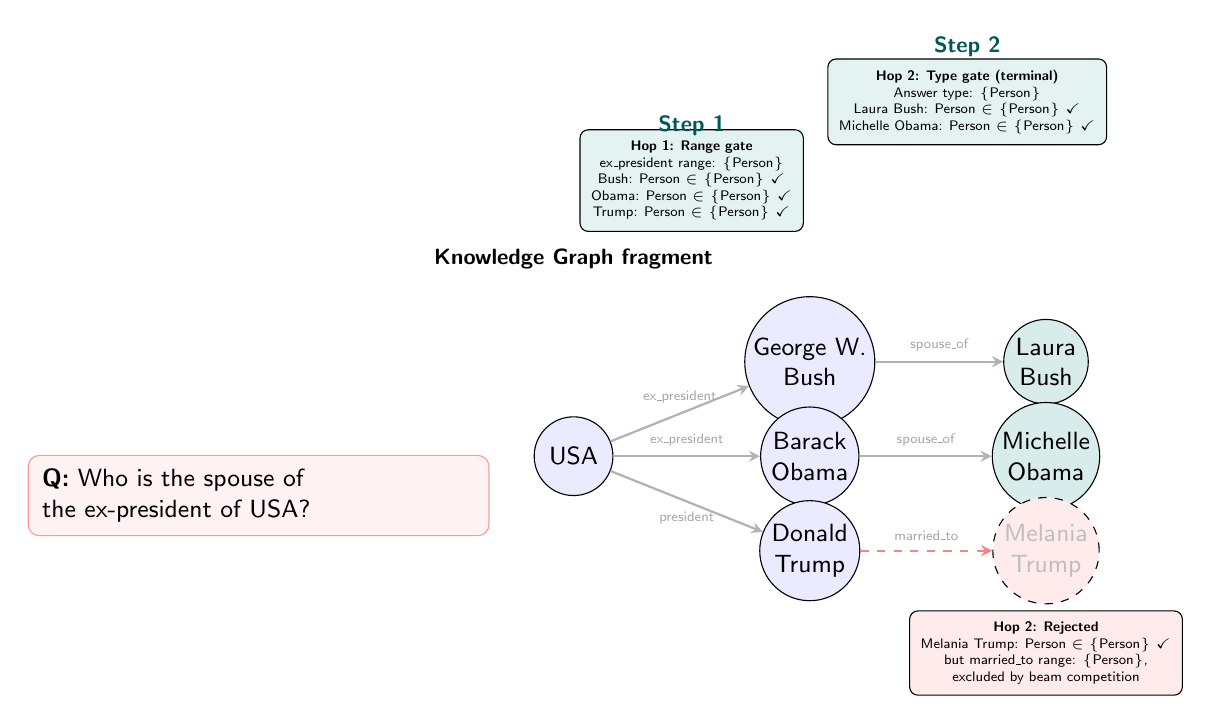
\begin{tikzpicture}[
  >=stealth, font=\sffamily,
  entity/.style={circle, draw, fill=blue!8, minimum size=1.0cm, inner sep=1pt,
    font=\sffamily\small, align=center},
  rel/.style={font=\sffamily\tiny, text=gray!70},
  accepted/.style={circle, draw, fill=teal!15, minimum size=1.0cm, inner sep=1pt,
    font=\sffamily\small, align=center},
  rejected/.style={circle, draw, dashed, fill=red!8, text=gray!50, minimum size=1.0cm,
    inner sep=1pt, font=\sffamily\small, align=center},
  gate/.style={draw, fill=yellow!15, rounded corners=3pt, inner sep=4pt,
    font=\sffamily\tiny, align=center},
  arr/.style={->, thick, draw=gray!60},
  rarr/.style={->, thick, draw=red!50, dashed},
  tarr/.style={->, thick, draw=teal!70!black},
]

  % Knowledge Graph (shifted down to clear title band)
  \node[font=\sffamily\footnotesize\bfseries] at (3, 0.5) {Knowledge Graph fragment};

  % Question
  \node[draw=red!40, fill=red!5, rounded corners=4pt, inner sep=5pt,
    font=\sffamily\small, align=left, text width=5.5cm]
    at (-1, -2.5) {\textbf{Q:} Who is the spouse of\\the ex-president of USA?};

  % Entities (shifted down)
  \node[entity] (usa) at (3, -2) {USA};
  \node[entity] (gwb) at (6, -0.8) {George W.\\Bush};
  \node[entity] (bo) at (6, -2) {Barack\\Obama};
  \node[entity] (dt) at (6, -3.2) {Donald\\Trump};
  \node[accepted] (lb) at (9, -0.8) {Laura\\Bush};
  \node[accepted] (mo) at (9, -2) {Michelle\\Obama};
  \node[rejected] (mt) at (9, -3.2) {Melania\\Trump};

  % Relations
  \draw[arr] (usa) -- node[above, rel] {ex\_president} (gwb);
  \draw[arr] (usa) -- node[above, rel] {ex\_president} (bo);
  \draw[arr] (usa) -- node[below, rel] {president} (dt);
  \draw[arr] (gwb) -- node[above, rel] {spouse\_of} (lb);
  \draw[arr] (bo) -- node[above, rel] {spouse\_of} (mo);
  \draw[rarr] (dt) -- node[above, rel] {married\_to} (mt);

  % Gate annotations (pushed higher, away from entities)
  \node[gate, fill=teal!10] at (4.5, 1.5) {
    \textbf{Hop 1: Range gate}\\
    ex\_president range: \{Person\}\\
    Bush: Person $\in$ \{Person\} \checkmark\\
    Obama: Person $\in$ \{Person\} \checkmark\\
    Trump: Person $\in$ \{Person\} \checkmark
  };

  \node[gate, fill=teal!10] at (8, 2.5) {
    \textbf{Hop 2: Type gate (terminal)}\\
    Answer type: \{Person\}\\
    Laura Bush: Person $\in$ \{Person\} \checkmark\\
    Michelle Obama: Person $\in$ \{Person\} \checkmark
  };

  \node[gate, fill=red!8] at (9, -4.5) {
    \textbf{Hop 2: Rejected}\\
    Melania Trump: Person $\in$ \{Person\} \checkmark\\
    but married\_to range: \{Person\},\\
    excluded by beam competition
  };

  % Step labels
  \node[font=\sffamily\footnotesize\bfseries, text=teal!70!black] at (4.5, 2.2) {Step 1};
  \node[font=\sffamily\footnotesize\bfseries, text=teal!70!black] at (8, 3.2) {Step 2};

\end{tikzpicture}
\end{document}
